\documentclass{ximera}

\title{Adding up Pieces: Double Integrals}
\author{Zack Reed}

\begin{document}
\begin{abstract}
In this activity we extend single-variable integration to functions of two variables, exploring double integrals over rectangular and general regions, Fubini's Theorem, and polar coordinates for curved regions.
\end{abstract}
\maketitle


\section*{Double Integrals for Volume}

An easily visualized interpretation of double integrals is computing volume under a surface.

\begin{definition}
For a function $f(x,y) \geq 0$ over a region $R$ in the $xy$-plane, the \textbf{double integral}
$$V = \iint_R f(x,y)\,dA = \iint_R f(x,y)\,dx\,dy$$
represents the volume between the surface $z=f(x,y)$ and the region $R$.
\end{definition}

\begin{problem}

When we plot simply in cartesian coordinates, the domain $dA=dx\,dy$ is a small rectangle.

When we use a double integral, we add up little products $f\cdot dx\,dy$. We can interpret $f$ as a height, and $dx\,dy$ as a small area element. So $f\cdot dx\,dy$ is like a tiny rectangular box with volume $f\cdot dx\,dy$.

\begin{expandable}{stuff}{GeoGebra Instructions}
    Alter the rectangle dimensions by dragging the top right corner. Change grid fineness with the sliders. Select a specific area element $dA$ to see the corresponding volume approximation $dV = f(a,b) \cdot dA$.
\end{expandable}

\begin{center}
\geogebra{yukegeqk}{755}{628}
\end{center}

Now let's explore some visual intuitions.

The number of dimensions in the \wordChoice{\choice{output}\choice[correct]{input}} of a function determines how many integrals we need to sum over.

Each small input piece $dA$ can be visually interpreted as having a measure of \wordChoice{\choice{length}\choice[correct]{area}\choice{volume}}.

The differentials $dx$ and $dy$ represent tiny \wordChoice{\choice[correct]{lengths}\choice{areas}\choice{volumes}} in the $x$ and $y$ directions, respectively.

The product $f(x,y) \cdot dx\,dy$ can be thought of as a tiny \wordChoice{\choice{length}\choice{area}\choice[correct]{volume}} of a region under the surface at point $(x,y)$.

As the grid becomes finer (smaller $dA$), the approximation:
\begin{multipleChoice}
    \choice{Gets worse}
    \choice[correct]{Gets better and approaches the true volume}
    \choice{Gets better and equals the true volume for some finite grid size}
    \choice{Stays the same}
    \choice{Oscillates}
\end{multipleChoice}

\end{problem}



\section*{Non-Rectangular Regions}

For non-rectangular regions, the bounds of integration become functions.

\begin{problem}
Find the volume under $f(x,y) = x + y$ over the triangular region with vertices $(0,0)$, $(1,0)$, $(1,1)$.

Even though the region is not rectangular, we can still use functions of $x$ and $y$ to describe the bounds of integration.

In this case, if we say that $x$ goes from 0 to 1, then for each fixed $x$, $y$ goes from 0 up to the line connecting $(0,0)$ and $(1,1)$, which has equation $y = x$.

So, the region can be described as: $0 \leq x \leq 1$ and $0 \leq y \leq \answer{x}$.

Since $x$ is a constant with respect to $y$, if we're mainitaining the main idea of partially integrating iteratively across the domain, we can integrate across $y$ first, treating $x$ as a constant, then integrate across $x$.

With this in mind the double integral becomes:
$$V = \iint dV=\iint x+y\,dA=\int_0^1 \int_0^x (x+y)\,dy\,dx$$

We break this down into two steps, evaluating the ``inner'' integral and then the ``outer'' integral.

\textbf{Inner integral:}
$$\int_0^x (x+y)\,dy = \left[\answer{xy + \frac{y^2}{2}}\right]_0^x = x^2 + \frac{x^2}{2} = \answer{3x^2/2}$$

\textbf{Outer integral:}
$$\int_0^1 \frac{3x^2}{2}\,dx = \frac{3}{2} \cdot \left[\answer{\frac{x^3}{3}}\right]_0^1 = \frac{3}{2} \cdot \frac{1}{3} = \answer{1/2}$$

\begin{feedback}
When the region is not rectangular, the bounds of the inner integral often depend on the outer variable!
\end{feedback}
\end{problem}


\section*{Practice: Unpacking Differential Constructions}

Before we tackle 3D domains, let's practice carefully constructing differential elements for various scenarios.

\begin{problem}
\textbf{Population Density Over a Strange Region}

A city's population density (people per square kilometer) varies with position and is given by:
$$\rho(x,y) = \frac{100}{1+x^2+y^2} \text{ people/km}^2$$

The city occupies the region bounded by $y = x^2$ (below) and $y = 4$ (above).

%a tikz plot of the region
\begin{center}
\begin{tikzpicture}[scale=0.8]
    \draw[->] (-3,0) -- (3,0) node[right] {$x$};
    \draw[->] (0,-1) -- (0,5) node[above] {$y$};
    \draw[domain=-2:2, smooth, variable=\x, blue] plot ({\x}, {\x*\x}) node[below] {$y=x^2$};
    \draw[domain=-3:3, smooth, variable=\x, red] plot ({\x}, {4}) node[right] {$y=4$};
\end{tikzpicture}
\end{center}

\textbf{Step 1: Construct the differential element}

For a small rectangular area element with dimensions $dx$ by $dy$:

The small area is: $dA = dx\,dy$

The small population in this area is: $dP = \rho \cdot dA = \rho(x,y)\answer{dx\,dy}=\answer{\frac{100}{1+x^2+y^2}}\cdot\answer{dx\,dy}$

This represents:
\begin{multipleChoice}
    \choice{The total population}
    \choice{The population density}
    \choice[correct]{The population in a tiny rectangular region}
    \choice{The average density}
\end{multipleChoice}

\textbf{Step 2: Determine integration bounds}

The region is bounded by $y = x^2$ below and $y = 4$ above.

%a tikz plot of th e region with a vertical slice at x=.5
\begin{center}
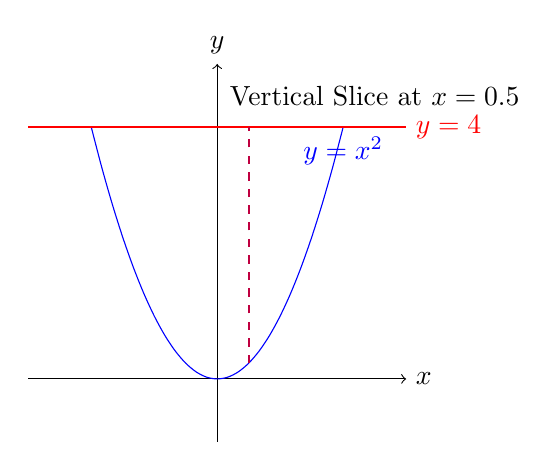
\begin{tikzpicture}[scale=0.8]
    \draw[->] (-3,0) -- (3,0) node[right] {$x$};
    \draw[->] (0,-1) -- (0,5) node[above] {$y$};
    %put the label on the bottom side of the graph
    \draw[domain=-2:2, smooth, variable=\x, blue] plot ({\x}, {\x*\x}) node[below] {$y=x^2$};
    \draw[domain=-3:3, smooth, variable=\x, red] plot ({\x}, {4}) node[right] {$y=4$};
    \draw[thick, dashed, purple] (0.5,0.25) -- (0.5,4);
    \node at (2.5,4.5) {Vertical Slice at $x=0.5$};
\end{tikzpicture}
\end{center}

For a vertical slice at position $x$, $y$ ranges from $\answer{x^2}$ to $\answer{4}$.

%a tikz plot of the region showing the intersection points of y=x^2 and y=4 as big dots
\begin{center}
\begin{tikzpicture}[scale=0.8]
    \draw[->] (-3,0) -- (3,0) node[right] {$x$};
    \draw[->] (0,-1) -- (0,5) node[above] {$y$};
    \draw[domain=-2:2, smooth, variable=\x, blue] plot ({\x}, {\x*\x}) node[below] {$y=x^2$};
    \draw[domain=-3:3, smooth, variable=\x, red] plot ({\x}, {4}) node[right] {$y=4$};
    \fill[black] (-2,4) circle (3pt) node[above] {(?,4)};
    \fill[black] (2,4) circle (3pt) node[above] {(?,4)};
\end{tikzpicture}
\end{center}

To cover the entire region, we need $x$ from $\answer{-2}$ to $\answer{2}$ (where does $x^2 = 4$?).

\textbf{Step 3: Set up the integral}

Total population: 
$$P = \iint_R dP = \int_{-2}^{2} \int_{x^2}^{4} \frac{\answer{100}}{1+x^2+y^2}\,dy\,dx$$

The order of integration matters because:
\begin{multipleChoice}
    \choice{The density function is complicated}
    \choice[correct]{The region is easier to describe with vertical slices (fixed $x$, varying $y$)}
    \choice{It always matters}
    \choice{We need to use Fubini's Theorem}
\end{multipleChoice}

\begin{feedback}
Excellent! You've carefully unpacked $dP = \rho(x,y)\,dA$ and set up bounds for a non-rectangular region. The density function decreases as you move away from the origin—the city center is most densely populated!
\end{feedback}
\end{problem}


What we've practiced with 2D regions can really be applied to any higher dimensional input space. Next section we'll apply these ideas for 3D regions, and then we'll see how to adapt our approach for curved regions as well.

\end{document}